%
% $Id: $
%
%
% Compilar a .pdf con LaTeX (pdflatex)
% Es necesario instalar Beamer (paquete latex-beamer en Debian)
%

%
% Gr�ficos:
% Los gr�ficos pueden suministrarse en PNG, JPG, TIF, PDF, MPS
% Los EPS deben convertirse a PDF (usar epstopdf)
%

\documentclass{beamer}
\usetheme{Warsaw}
%\usebackgroundtemplate{
\includegraphics[width=\paperwidth]{format/libresoft-bg.png}}
%\usepackage[spanish]{babel}
\usepackage[latin1]{inputenc}
\usepackage{graphics}
\usepackage{amssymb} % Simbolos matematicos
\usepackage{url}

%\definecolor{libresoftgreen}{RGB}{162,190,43}
%\definecolor{libresoftblue}{RGB}{0,98,143}

%\setbeamercolor{titlelike}{bg=libresoftgreen}

%% Metadatos del PDF.
\hypersetup{
  pdftitle={Developing Mathematical Thinking with Scratch: An Experiment with 6th Grade Students},
  pdfauthor={Luis Alberto Calao, Jes�s Moreno Le�n, Heidy Ester Correa, Gregorio Robles},
  pdfcreator={GSyC/LibreSoft \\ Universidad Rey Juan Carlos},
  pdfproducer=PDFLaTeX,
  pdfsubject={Computational Thinking. Mathematics. Programming. Scratch},
}
%%

\begin{document}

\title{Developing Mathematical Thinking with Scratch}
\subtitle{An Experiment with 6th Grade Students}
\institute{jesus.moreno@programamos.es, grex@gsyc.urjc.es \\
GSyC/Libresoft, Universidad Rey Juan Carlos}
\author{Luis Alberto Calao, Jes�s Moreno Le�n, Heidy Ester Correa, Gregorio Robles}
\date{EC-TEL 2015, Toledo}

\frame{
\maketitle
\begin{center}

\includegraphics[width=2cm]{format/libresoft-logo}
\hspace{0.5cm}

\includegraphics[width=5cm]{format/gsyc-urjc}
\vspace{0.5cm}

\includegraphics[width=3cm]{format/emadrid.png}
\end{center}
}


% Si el titulo o el autor se quieren acortar para los pies de p�gina
% se pueden redefinir aqu�:
%\title{Titulo corto}
%\author{Autores abreviado}

%% LICENCIA DE REDISTRIBUCION DE LAS TRANSPAS
\frame{
~
\vspace{3cm}

\begin{flushright}

\includegraphics[width=2.2cm]{figs/by-sa}

{\tiny
(cc) 2015 Gregorio Robles and Jes�s Moreno Le�n\\
  Some rights reserved. This work licensed under Creative Commons \\
  Attribution-ShareAlike License. To view a copy of full license, see \\
  http://creativecommons.org/licenses/by-sa/3.0/ or write to \\
  Creative Commons, 559 Nathan Abbott Way, Stanford, \\
  California 94305, USA. \\
\ \\
Some of the figures have been taken from the Internet \\
Source, and author and licence if known, is specified. \\
For those images, \emph{fair use} applies.
}
\end{flushright}
}
%%

\section{EC-TEL 2015, Toledo}


%--------------------------------------------------------
%\usebackgroundtemplate{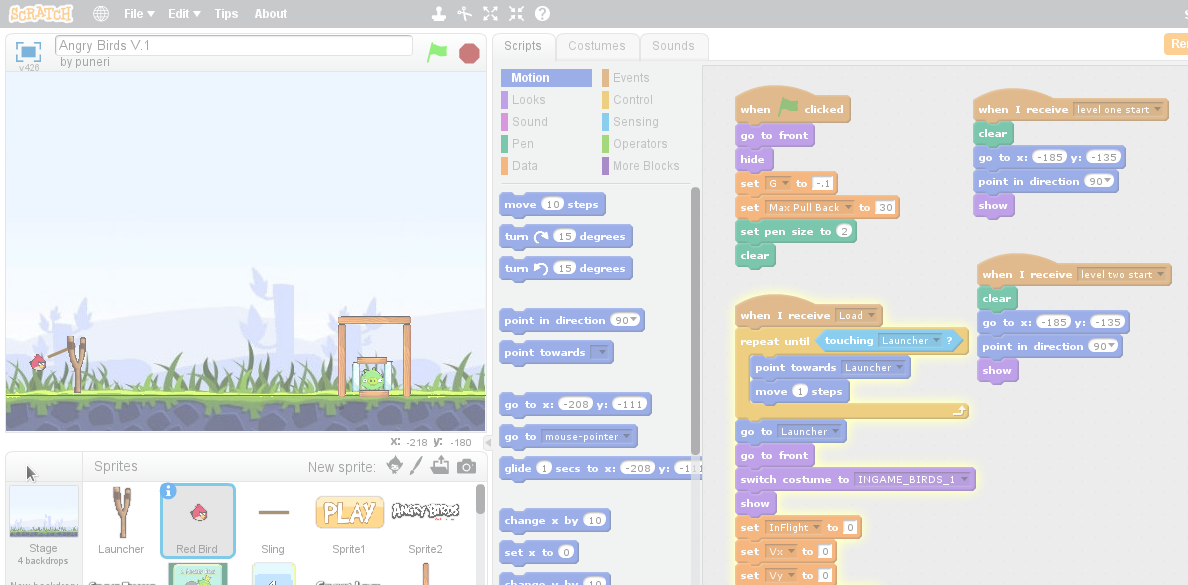
\includegraphics[width=18cm]{figs/AngryBirds.png}}

\begin{frame}
\frametitle{Goal of our paper}

\begin{center}
\Huge {\bf Does the use of programming with Scratch in math classes improve students' learning outcomes?}
\end{center}

\end{frame}

%--------------------------------------------------------
\usebackgroundtemplate{
\includegraphics[width=18cm]{figs/colombia.jpg}}

\begin{frame}
\frametitle{Colombian students and maths}
\begin{columns}[T]
  \begin{column}{1\textwidth}
     \begin{block}{PISA 2012 results}
       \begin{itemize}
	 \item 376 points in maths (OECD countries average: 494)
         \item Ranked 61st (out of 65 participating countries)
         \item Students showed high levels of anxiety towards maths
       \end{itemize}
    \end{block}
  \end{column}
\end{columns}
%\hfill{\Tiny Background picture: House of Colombia San Diego} 
\end{frame}

\usebackgroundtemplate{}

%--------------------------------------------------------
%\usebackgroundtemplate{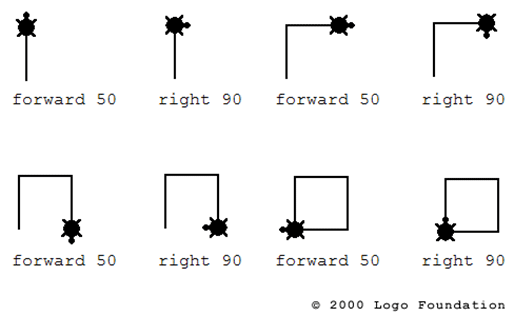
\includegraphics[height=10cm]{figs/turtles.png}}
% background: http://www.wim-network.org/wp-content/uploads/2012/04/iceberg.jpg

\begin{frame}
\frametitle{Code to learn (I)}
\begin{columns}[T]
  \begin{column}{0.5\textwidth}
    \begin{figure}[t!]
      \begin{center}
	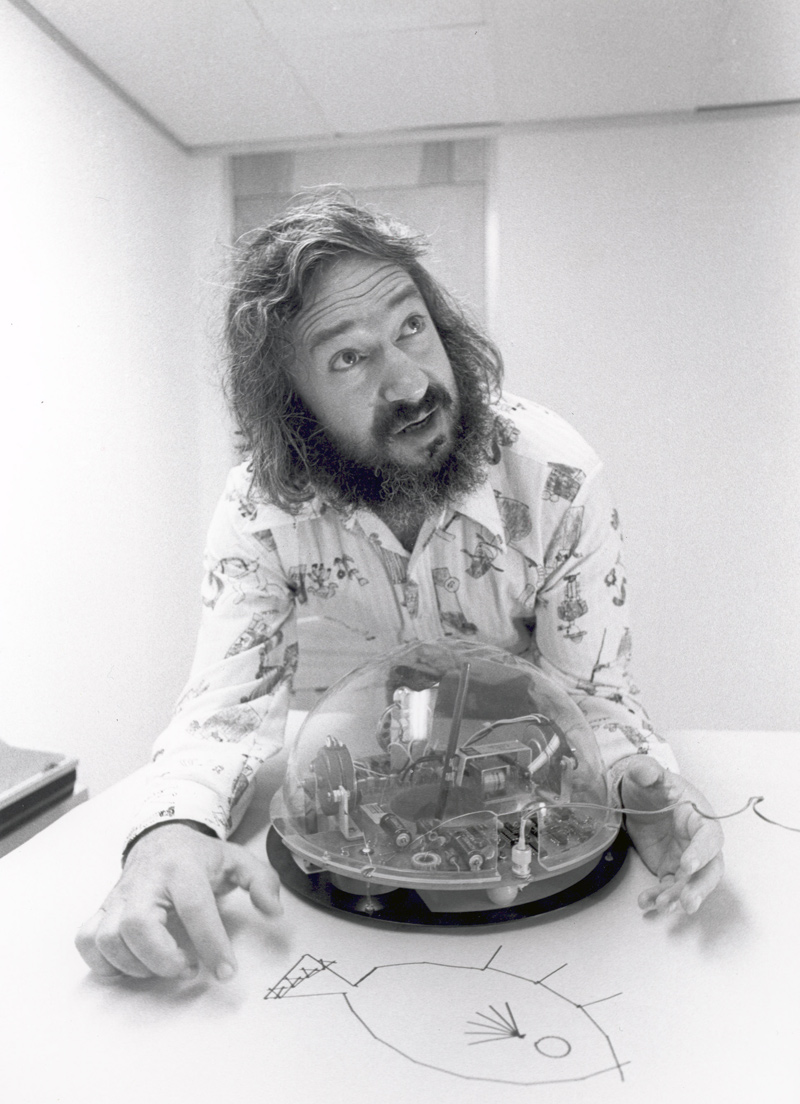
\includegraphics[width=5cm]{figs/seymour.jpg}
      \end{center}
      \label{fig:repetition1}
    \end{figure}
  \end{column}
  \begin{column}{0.5\textwidth}
    \begin{block}{Logo programming language}
      \begin{itemize}
	 \item Developed in the 1960s
         \item Its educational impact was intensively investigated in the 70s and 80s
         \item Students' improvements in maths (and other disciplines) were proved
         \item ``Disappeared'' from the educational landscape since mid-90s
      \end{itemize}
    \end{block}
    \hfill{\Tiny Seymour Papert's picture: jgora.net}
  \end{column}
\end{columns}
\end{frame}

\usebackgroundtemplate{}

%--------------------------------------------------------
\usebackgroundtemplate{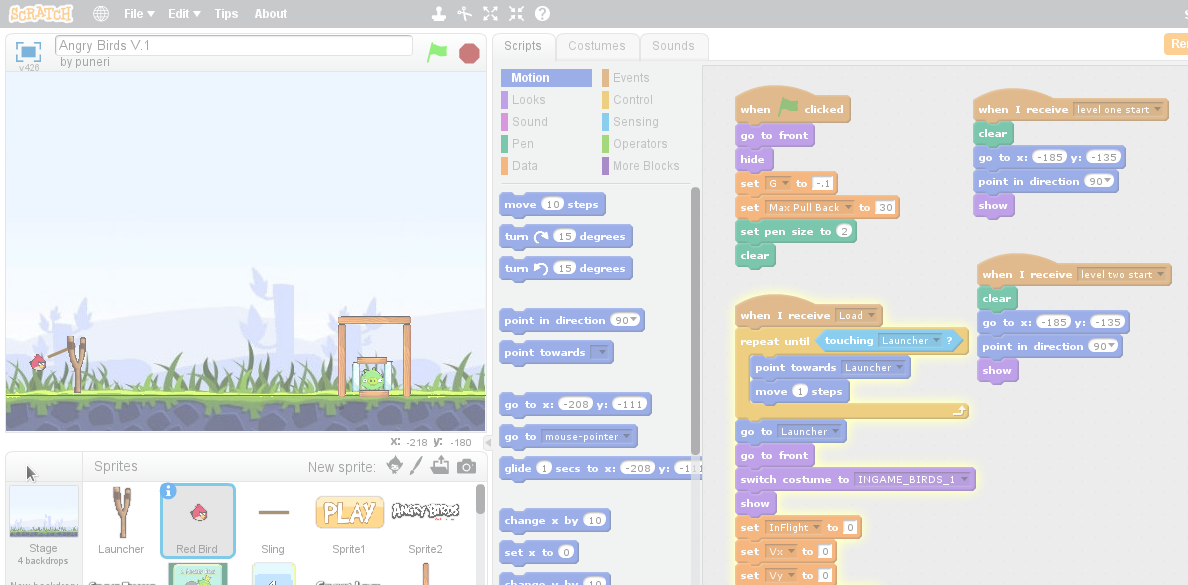
\includegraphics[width=18cm]{figs/AngryBirds.png}}
\begin{frame}
\frametitle{Code to learn (and II)}

\begin{columns}[T]
  \begin{column}{1\textwidth}
     \begin{block}{New visual programming languages}
       \begin{itemize}
	 \item Alice, Kodu, Scratch
         \item Very promising research literature 
         \item There is need for empirical studies
       \end{itemize}
    \end{block}
  \end{column}
\end{columns}

\end{frame}
\usebackgroundtemplate{}
%--------------------------------------------------------
\usebackgroundtemplate{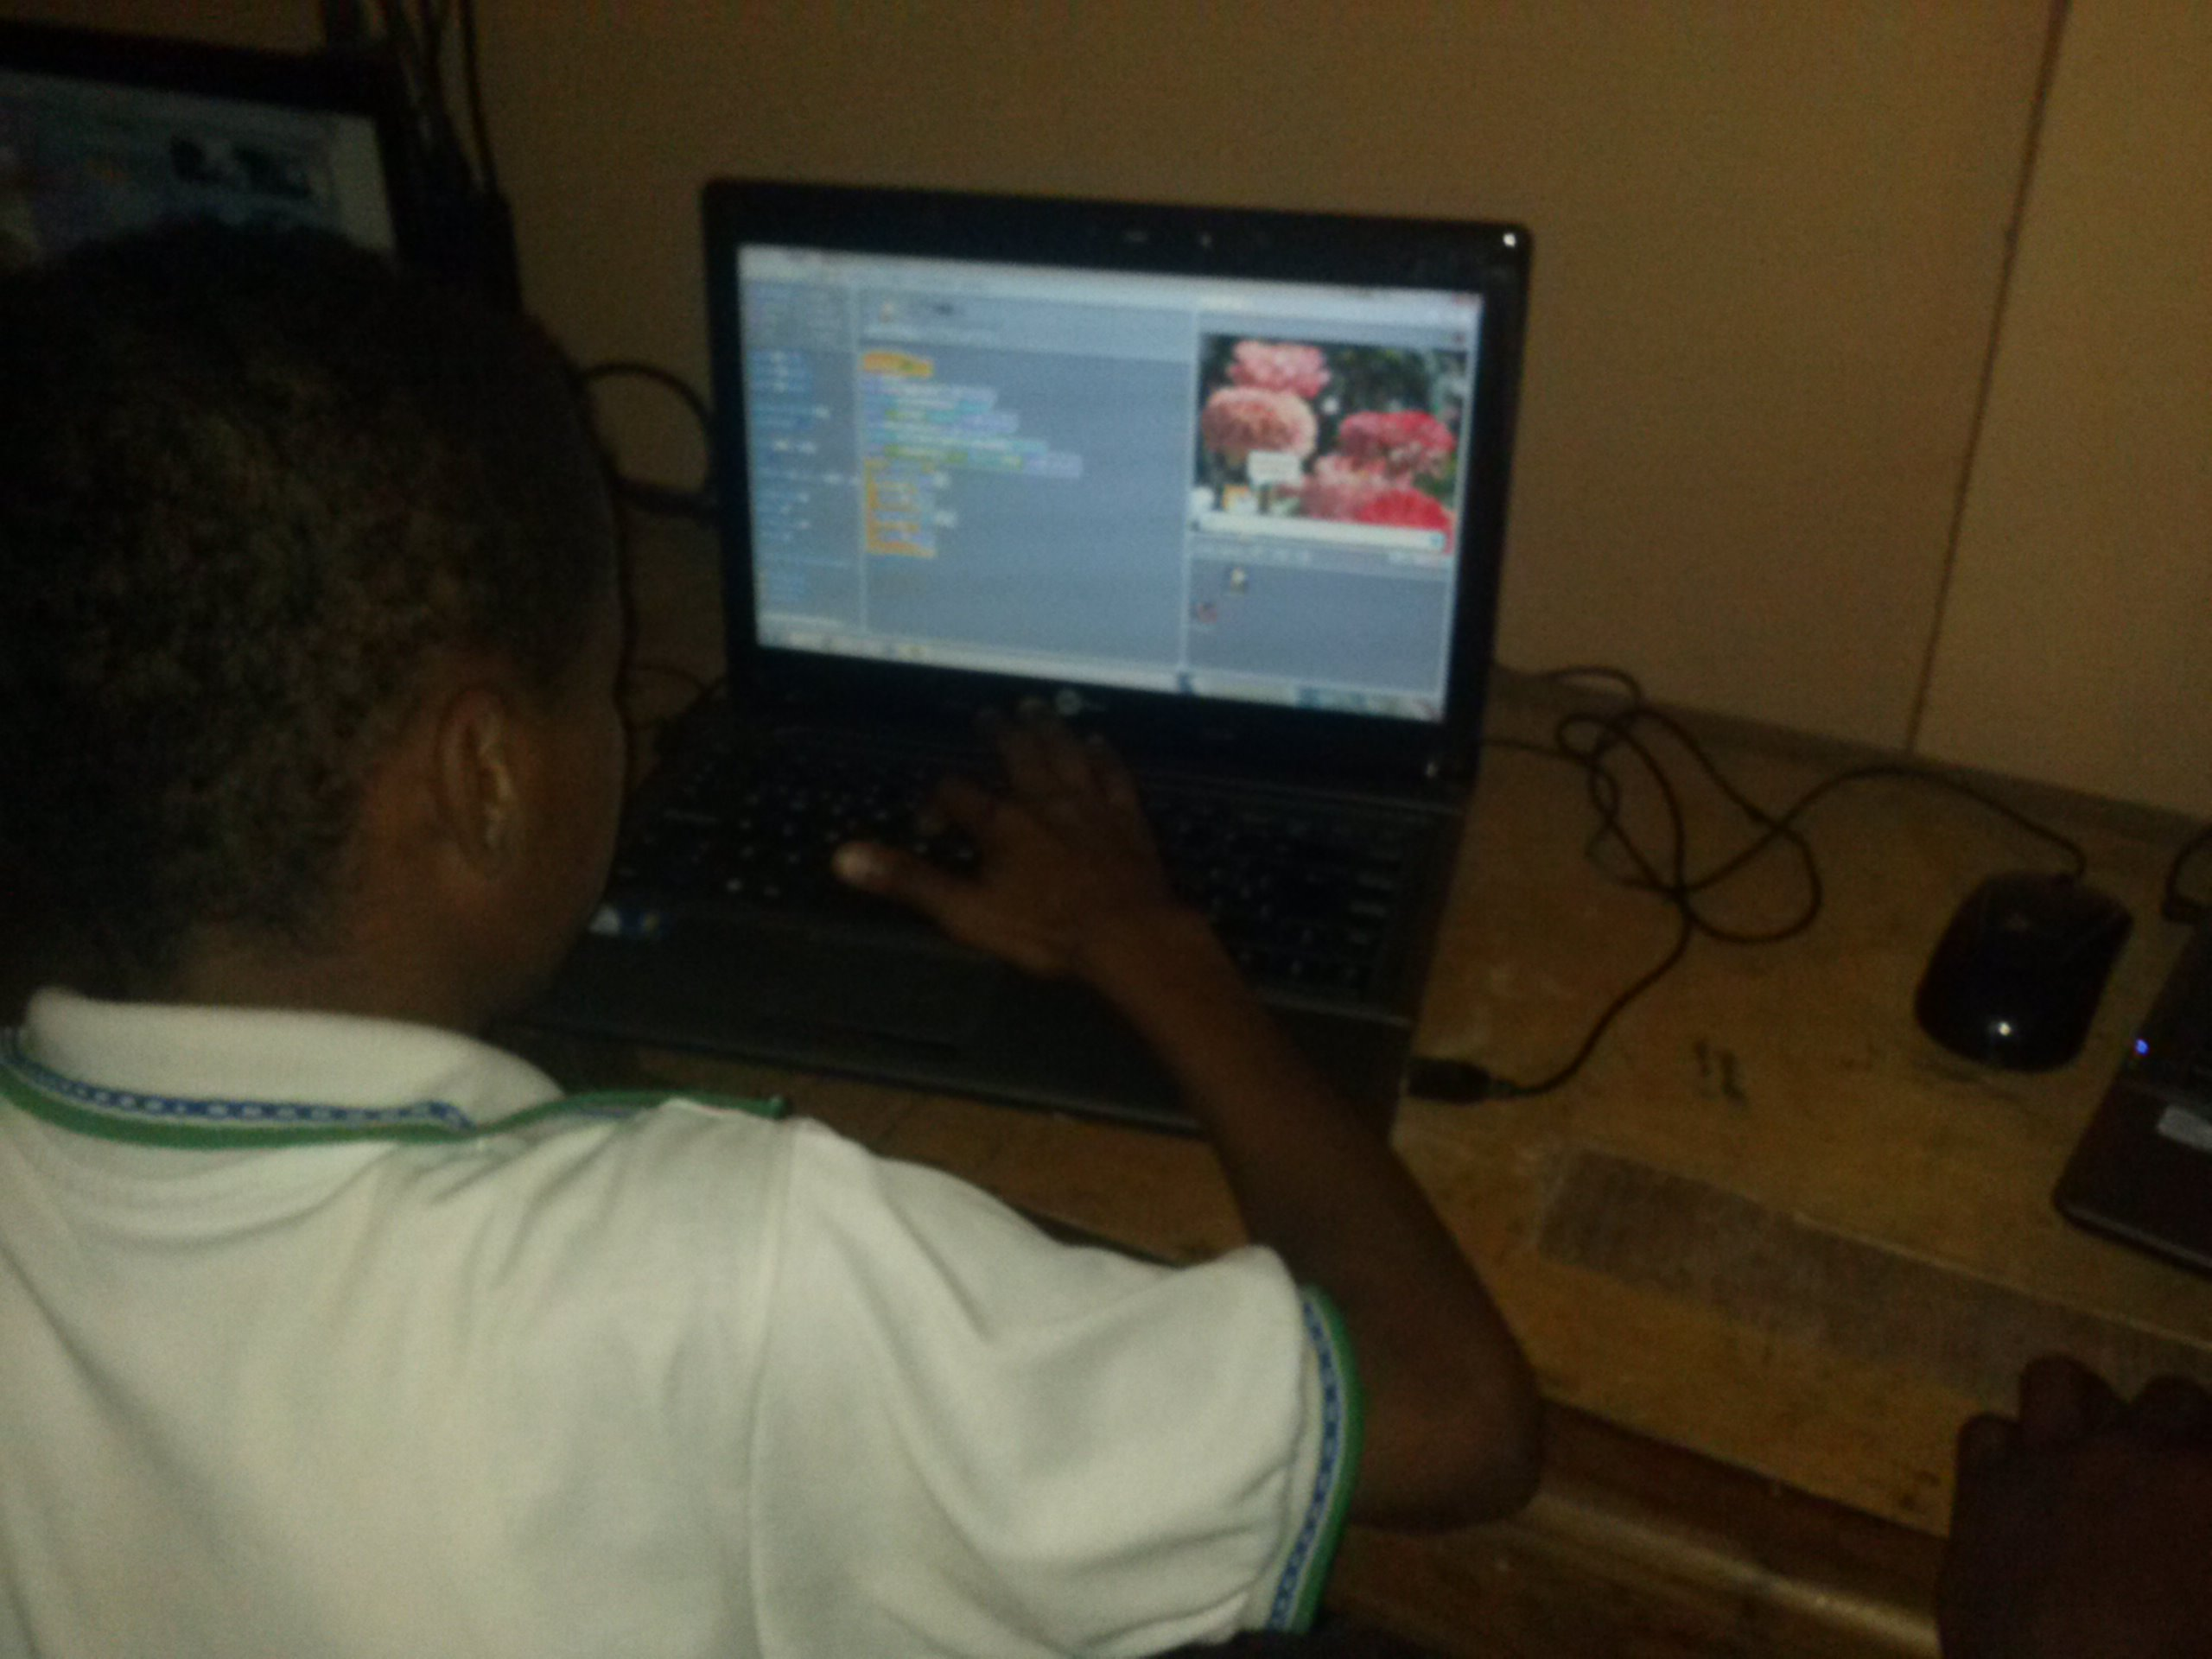
\includegraphics[width=13cm,height=9.2cm]{figs/coding.jpg}}
\begin{frame}
\frametitle{The study}


  \begin{columns}[T]
    \begin{column}{1\textwidth}
     \begin{block}{Code to learn Maths with Scratch}
\begin{itemize}
  \item Quasi-Experimental Design
  \item 42 students, 6\textsuperscript{th} grade
  \item Control groups and experimental groups
  \item Pre and Post tests
  \item 3 months
\end{itemize}
    \end{block}
    \end{column}
    
  \end{columns}

\end{frame}

\usebackgroundtemplate{}

%--------------------------------------------------------
\usebackgroundtemplate{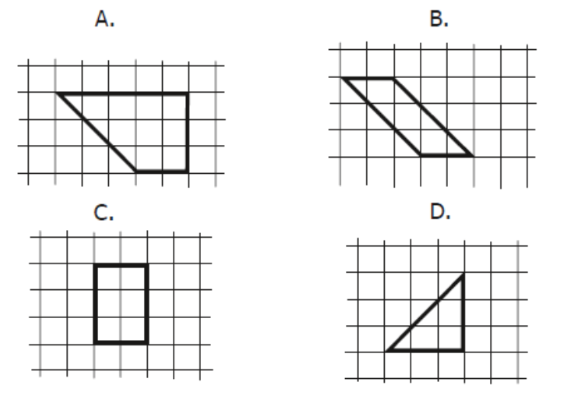
\includegraphics[width=13cm,height=9.2cm]{figs/rubric.png}}
\begin{frame}
\frametitle{Mathematical processes investigated}
\begin{columns}[T]
    \begin{column}{0.8\textwidth}
     \begin{block}{Rubric}
\begin{itemize}
  \item Modeling of processes and reality phenomena
  \item Reasoning (making predictions and justifying arguments)
  \item Problem formulation and problem solving
  \item Exercising (comparison and execution of procedures and algorithms)
  \item Following guidelines set by the Ministry of National Education of Colombia
\end{itemize}
    \end{block}
    \end{column}
  \end{columns}
\end{frame}

\usebackgroundtemplate{}
%--------------------------------------------------------
\begin{frame}
\frametitle{Results (I)}

\begin{figure}[t!]
\begin{center}
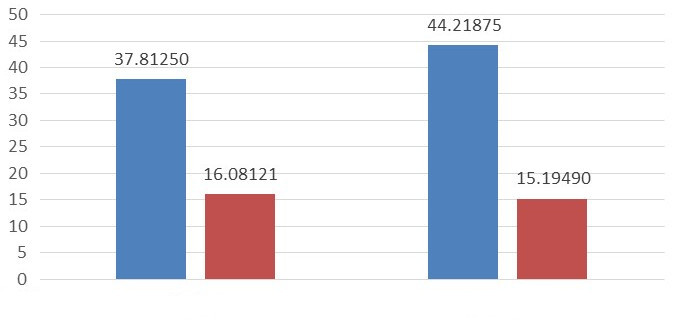
\includegraphics[width=9cm]{figs/pre.jpg}
\end{center}
\label{fig:naming}
\end{figure}

\begin{center}
Pre-test. Mean and deviation for control (left) and experimental (right) groups.
\end{center}
\end{frame}

\usebackgroundtemplate{}

%--------------------------------------------------------
\begin{frame}
\frametitle{Results (II)}

\begin{figure}[t!]
\begin{center}
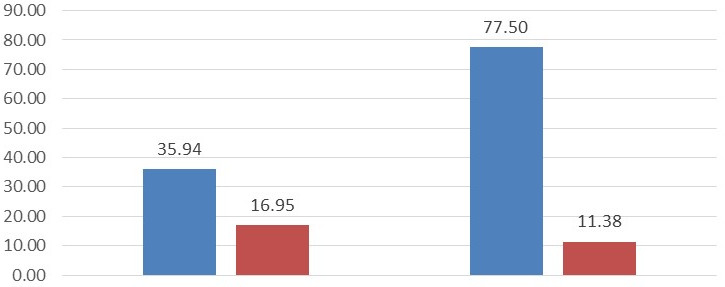
\includegraphics[width=9cm]{figs/post.jpg}
\end{center}
\label{fig:naming}
\end{figure}

\begin{center}
Post-test. Mean and deviation for control (left) and experimental (right) groups.
\end{center}
\end{frame}

\usebackgroundtemplate{}

%--------------------------------------------------------
\begin{frame}
\frametitle{Results (and III)}

\begin{figure}[t!]
\begin{center}
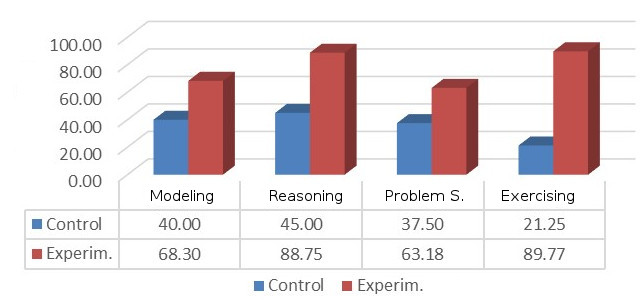
\includegraphics[width=9cm]{figs/comparison.jpg}
\end{center}
\label{fig:naming}
\end{figure}

\begin{center}
Post-test comparison. Means obtained for the control and experimental groups by mathematical process.
\end{center}
\end{frame}

\usebackgroundtemplate{}

%--------------------------------------------------------
%\usebackgroundtemplate{
\includegraphics[width=13cm,height=9cm]{figs/take-away.jpg}}
% background: http://2.bp.blogspot.com/-78Eh4TBpdtU/UPw7ULV73PI/AAAAAAAAHAE/6DQfvPNCo-Y/s1600/8723052-stylized-red-stamp-showing-the-term-take-away-all-on-white-background.jpg

\begin{frame}
\frametitle{Conclusions}

\begin{itemize}
  \item The development of CT using Scratch allows students of primary education to improve their performance in terms of
mathematical processes of modeling, reasoning, problem solving and exercising.
  \item (At least some parts of) the math curriculum in Colombian schools does not help in developing these skills.
  \item Math learning at schools seems to be more focused on the internals of mathematics, rather than on acquiring skills to use math-based knowledge.
\end{itemize}
\vspace{\baselineskip}
\vspace{\baselineskip}

\end{frame}

\usebackgroundtemplate{}
%--------------------------------------------------------
\usebackgroundtemplate{
\includegraphics[width=13cm]{figs/future.png}}

\begin{frame}
\frametitle{Future Work}

\begin{enumerate}
  \item Does computer programming foster reading and writing skills?
  \item Programming with Scratch as an educational tool in different subjects (social studies, language arts) and grades.
  \item OK, but do the students really learn to code and develop computational thinking?
\end{enumerate}
\vspace{\baselineskip}
\vspace{\baselineskip}
\hfill{\Tiny Background picture: Simon Cunningham }

\end{frame}

\usebackgroundtemplate{}
%--------------------------------------------------------

\usebackgroundtemplate{
\includegraphics[width=13cm]{figs/future.png}}

\begin{frame}
\frametitle{Future Work}

\begin{figure}[t!]
\begin{center}
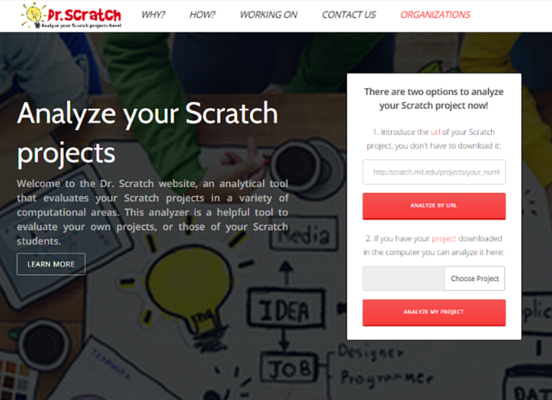
\includegraphics[width=9cm]{figs/drscratch1.png}
\end{center}
\label{fig:naming}
\end{figure}
\vspace{\baselineskip}
\vspace{\baselineskip}
\hfill{\Tiny Background picture: Simon Cunningham }

\end{frame}

\usebackgroundtemplate{}

%--------------------------------------------------------
\frame{
\maketitle
\begin{center}

\includegraphics[width=2cm]{format/libresoft-logo}
\hspace{0.5cm}

\includegraphics[width=5cm]{format/gsyc-urjc}
\vspace{0.5cm}

\includegraphics[width=3cm]{format/emadrid.png}
\end{center}
}

\end{document}
